\documentclass{beamer}
\usepackage[T1]{fontenc}
\usepackage[utf8]{inputenc}
\usepackage{lmodern}
\usepackage[brazil]{babel}
\usepackage[labelformat=empty]{caption}
\usepackage{multicol}
\usetheme{JuanLesPins}

\title{
       \textbf{Dojo de programação} \\
       CCSL - IME - USP
      }

\begin{document}
\maketitle
\section{Introdução}

\begin{frame}
  \frametitle{Mas o que é dojo?}
  \framesubtitle{}
  
  \begin{figure}[htb]
    \begin{center}
      
\includegraphics[scale=0.5]{jack.jpg}
    \end{center}
  \end{figure}
\end{frame}

\begin{frame}
  \frametitle{Dojo é:}
  \framesubtitle{}
  \begin{figure}[htb]
    \begin{center}
      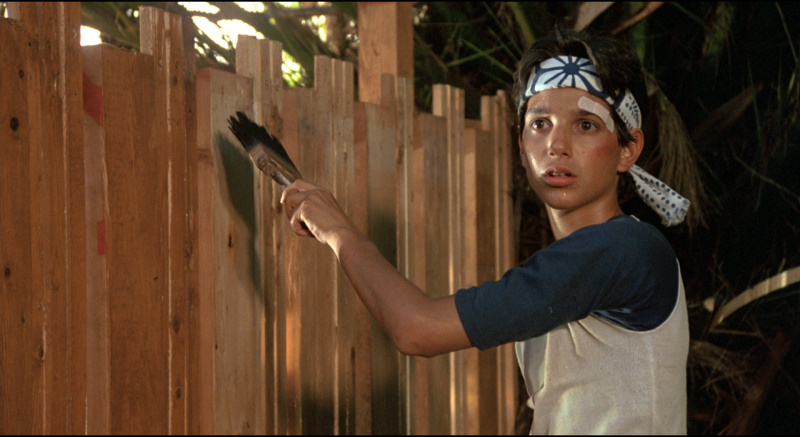
\includegraphics[scale=0.35]{puxo.jpg}
      \caption{O \textbf{treinamento} de um programador.}
    \end{center}
  \end{figure}
\end{frame}

\begin{frame}
  \frametitle{Dojo é:}
  \framesubtitle{}
  A alma de um dojo de programação é essa:
  \begin{itemize}
    \item Escrever o \textbf{melhor} código que você puder;
    \item \textbf{Não ter compromisso} de finalizar;
    \item Trocar \textbf{experiências} com outros programadores;
    \item Ter contato com \textbf{novas tecnologias}.
  \end{itemize}
\end{frame}

\begin{frame}
  \frametitle{Funciona assim...}

  \begin{itemize}
    \item Um monte de \textbf{programadores} (ou curiosos) se juntam;
    \item Escolhem um \textbf{desafio} (ou tema) sobre o qual querem aprender;
    \item \textbf{Pares} programam enquanto os demais prestam atenção na solução sendo implementada;
      \begin{itemize}
        \item \textbf{Rotação}: O par é trocado a cada poucos minutos;
        \item \textbf{Testes}: Queremos código de qualidade, então fazemos TDD (Test-Driven Development);
        \item \textbf{Não} há obrigação de \textbf{finalizar} o desafio.
      \end{itemize}
    \item Depois que encerramos, conversamos sobre como foi tudo e como podemos \textbf{melhorar}.
  \end{itemize}
\end{frame}

\section{Temas}
\begin{frame}
  \frametitle{Escolha do desafio}

  \begin{enumerate}
    \item Internacionalização com RoR (Ruby on Rails)
    \item Criação de modelos sem ActiveRecord no RoR
    \item Lançamento de uma gema do Ruby
    \item Criação de gráficos em Ruby com gruff
    \item CoffeeScript \& Ajax
    \item Testes automatizados
  \end{enumerate}
\end{frame}

\begin{frame}
  \frametitle{Escolha do desafio}
  \framesubtitle{1. Internacionalização}
  \begin{figure}[htb]
    \begin{center}
      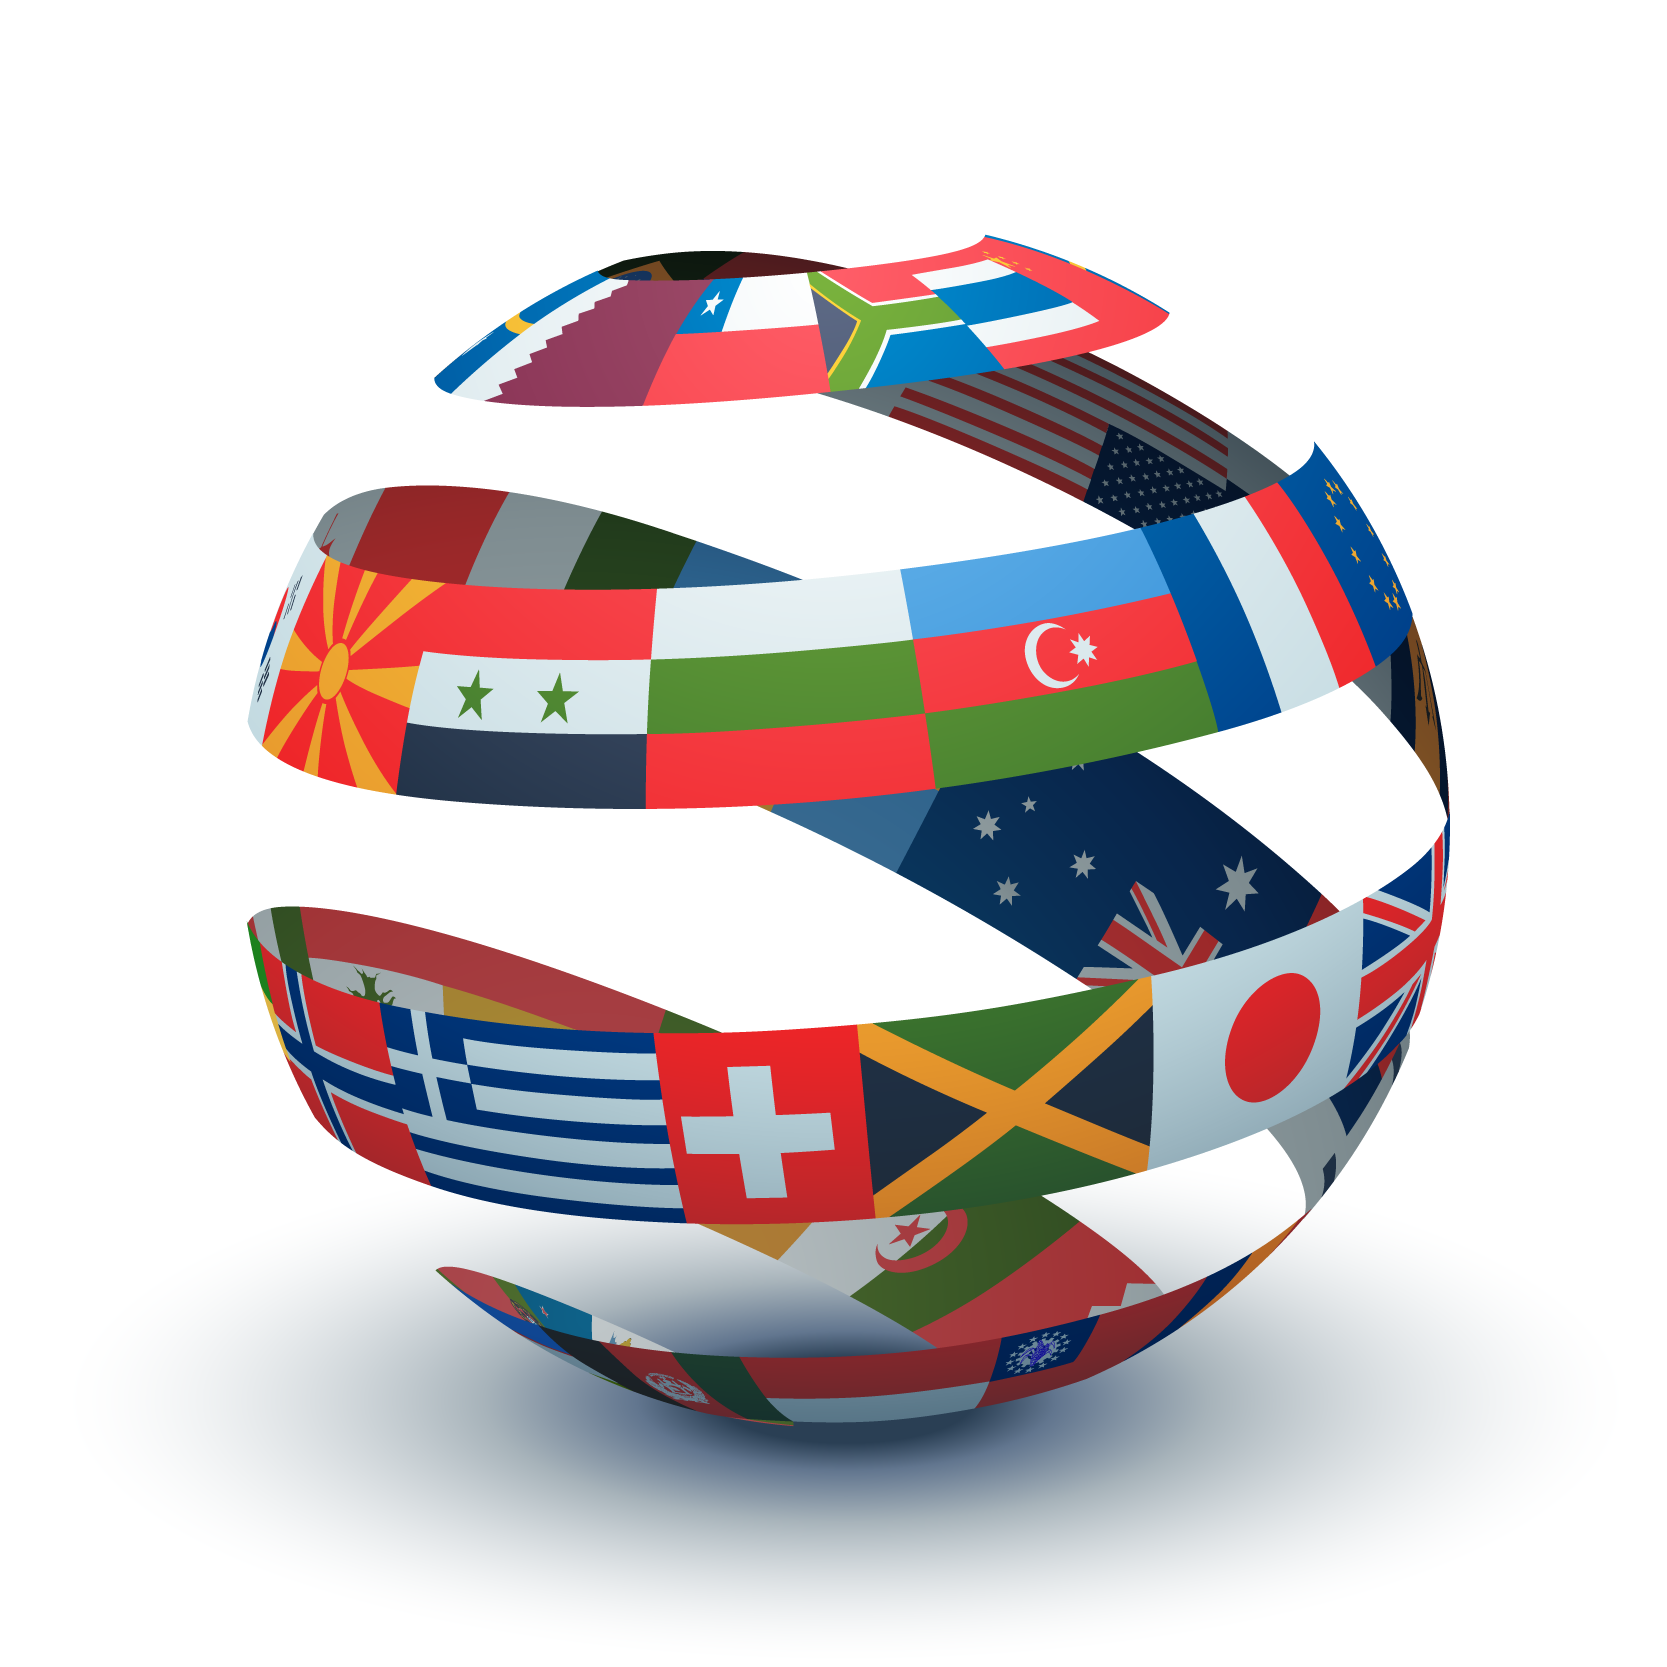
\includegraphics[scale=0.18]{small-globe.png}
    \end{center}
  \end{figure}

  Uma mesma aplicação pode ser acessada por pessoas com \textbf{diferentes preferências de idioma} além do inglês. \\~\\

  Então, pensando nisso, nossos amigos desenvolvedores do Rails incorpararam a gem \textbf{i18n} ao framework, facilitando nossa vida. \\~\\

  Que tal internacionalizarmos algumas partes do novo Mezuro?
\end{frame}

\begin{frame}
  \frametitle{Escolha do desafio}
  \framesubtitle{2. nonActiveRecord models}

  Em Rails todos os modelos clássicos herdam de uma classe chamada ActiveModel, parte da gem ActiveRecord que precisa de um banco de dados. \\~\\

  E se você \textbf{não} quiser um \textbf{banco de dados}, mas quer todas as outras coisas legais que um modelo do Rails tem? \\~\\

  \begin{multicols}{2}
    \begin{figure}[htb]
      \begin{center}
        
\includegraphics[scale=0.1]{no-database.png}
      \end{center}
    \end{figure}

    \columnbreak

    \begin{figure}[htb]
      \begin{center}
        
\includegraphics[scale=0.2]{rails.png}
      \end{center}
    \end{figure}
  \end{multicols}

  No Mezuro demos um jeito nisso! Quer ver o que fizemos e dar sugestões?
\end{frame}

\begin{frame}
  \frametitle{Escolha do desafio}
  \framesubtitle{3. Desenvolvimento de gems para Ruby}

  \begin{multicols}{2}
    \begin{figure}[htb]
      \begin{center}
        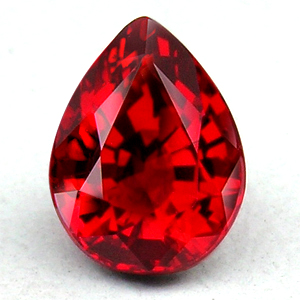
\includegraphics[scale=0.1]{ruby-gem.jpg}
      \end{center}
    \end{figure}

    \columnbreak
    
    Basicamente, uma gema é um pacote que encapsula uma funcionalidade. \\~\\
  \end{multicols}

  O Mezuro utiliza várias gemas que dão suporte à sua implementação desde testes até cadastramento de usuários, como por exemplo o devise, factoryGirl, rspec e o kalibro\_entities.\\~\\
  
  Em especial, o Kalibro é uma ferramenta utilizada pelo Mezuro para calcular métricas. Atualmente, nossa equipe está desenvolvendo uma gema para ela. \\~\\
  
  Então, vamos implementar uma das entidades do kalibro\_gem?

\end{frame}

\begin{frame}
	\frametitle{Escolha do desafio}
  \framesubtitle{4. Criação de gráficos em ruby com gruff}
  
  No Mezuro, utilizamos o \textbf{gruff} para plotar os gráficos.

  \begin{figure}[htb]
    \begin{center}
      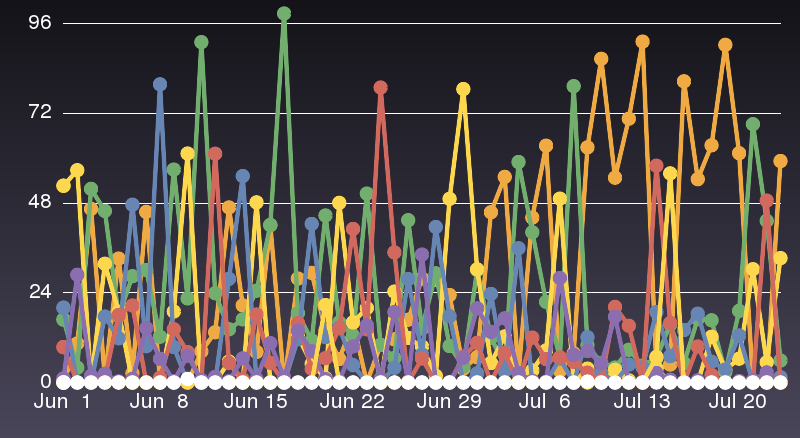
\includegraphics[scale=0.15]{graph.png}
    \end{center}
  \end{figure}
  
  Ele é uma gema que fornece suporte à criação de diversos tipos de gráficos. \\~\\
  Podemos aprender a gerar número aleatórios em Ruby para criar os dados ou podemos gerar gŕaficos para o Mezuro! \\~\\
  
  Alguém se anima em aprender a mexer no gruff?
\end{frame}

\begin{frame}
	\frametitle{Escolha do desafio}
  \framesubtitle{5. CoffeeScript \& Ajax}

  \begin{multicols}{3}
    \begin{figure}[htb]
      \begin{center}
        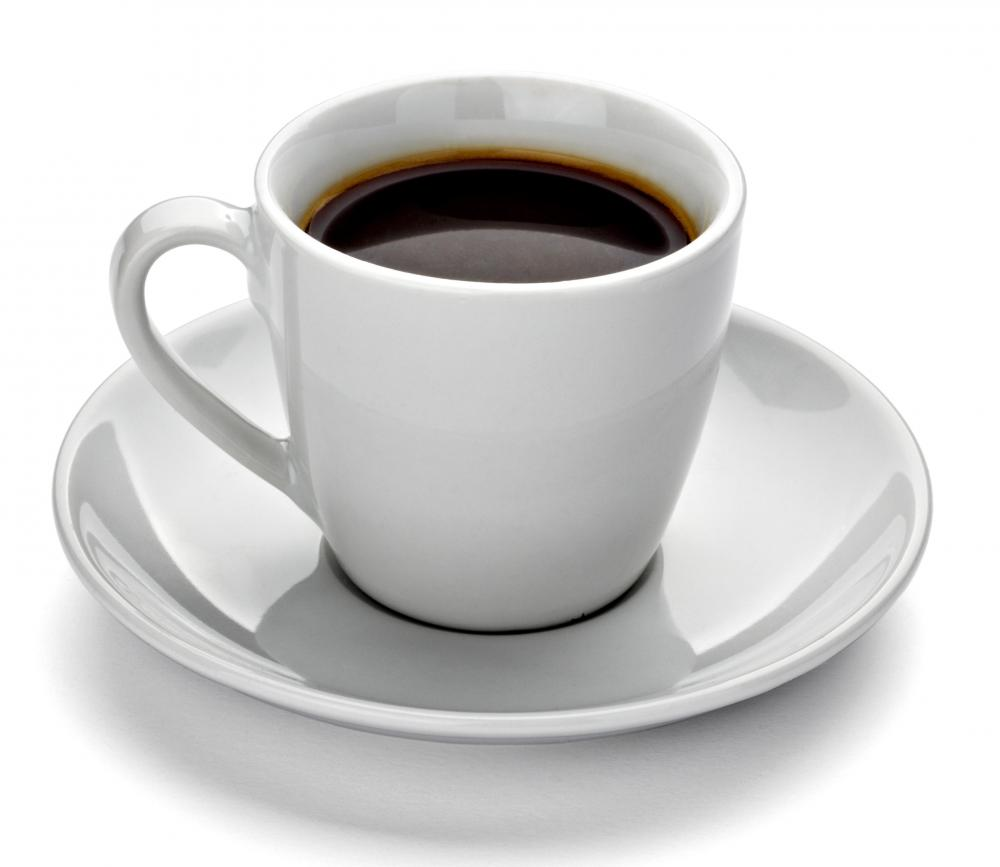
\includegraphics[scale=0.04]{coffee.jpg}
      \end{center}
    \end{figure}

    \columnbreak

    \begin{figure}[htb]
      \begin{center}
        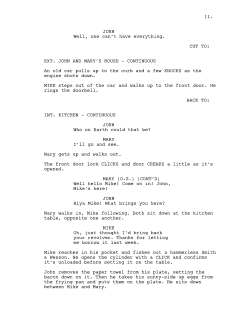
\includegraphics[scale=0.13]{script.png}
      \end{center}
    \end{figure}

    \columnbreak

    \begin{figure}[htb]
      \begin{center}
        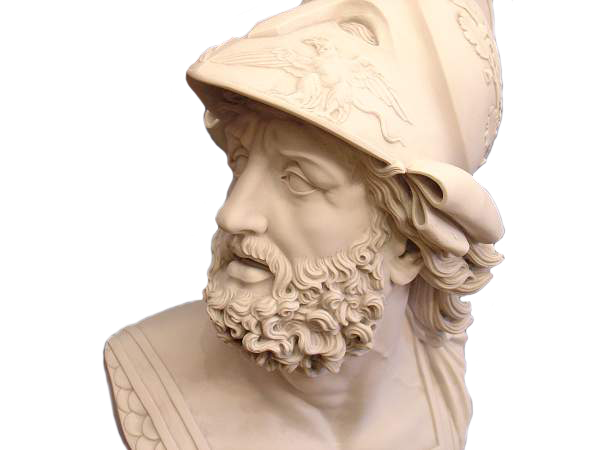
\includegraphics[scale=0.08]{ajax.png}
      \end{center}
    \end{figure}

  \end{multicols}
  
  \textbf{CoffeeScript} é uma linguagem que facilita o uso do \textbf{JavaScript}, que é a linguagem utilizada para deixar páginas web dinâmicas. \\~\\
  Já o \textbf{Ajax} é uma ferramenta para carregamento assíncrono de página. \\~\\
  As ferramentas mencionadas acima são usadas no Mezuro para mostrar resultados de processamento. \\~\\
  
  E aí, pessoal! Vamos nos familiarizar com estas ferramentas?
\end{frame}

\begin{frame}
	\frametitle{Escolha do desafio}
  \framesubtitle{6. Testes automatizados}

  \begin{figure}[htb]
    \begin{center}
      
\includegraphics[scale=0.2]{automation.jpg}
    \end{center}
  \end{figure}
  
  Testes automatizados servem para detectar  rapidamente  defeitos,  ajudar  no  controle de  qualidade  do  código  e  fornecem   uma  documentação  simples  das  funcionalidades  do sistema. \\~\\
  No Mezuro, utilizamos o \textbf{Cucumber} e o \textbf{Rspec} para fazer a cobertura dos testes de aceitação e unidade, respectivamente. \\~\\
  
  E aí, vamos aprender a fazer testes automatizados para o nosso programa?

\end{frame}

\begin{frame}
  \LARGE{\textbf{Vamos votar!}}
\end{frame}

\section{Atividade}
\begin{frame}
  \LARGE{\textbf{Hora de programar então!!!!!!}}
\end{frame}

\section{Retrospectiva}
\begin{frame}
  \frametitle{Retrospectiva}
  \framesubtitle{Foi bom para você?}

  \begin{itemize}
    \item É livre para você dizer o que quiser;
    \item Sugestões são muito bem vindas;
    \item E críticas são ainda mais!
  \end{itemize}
\end{frame}

\begin{frame}
  \LARGE{\textbf{ACABOU :(}} \\~\\

  Mantenha contato conosco:

  \textbf{team@kalibro.org}

  \textbf{GoogleGroups}: dojos-mezuro@googlegroups.com
\end{frame}
\end{document}
